\section{Experimental}

\subsection{Samples}

\begin{table}[H]
\centering
\begin{tabular}{|c|m{6cm}|c|}
\hline
\textbf{Name} & \textbf{Description} & \textbf{Feedstock} \\ \hline
R6-Q3-210 & Polysilicon, electronic grade, clean feedstock & Siemens process \\ \hline
ES1-Q3-201 & Large amount of P and B, solar grade, dirty feedstock & From Elkem \cite{hystad09} \\ \hline
MH2-Q3-201 & Same as ES1 with added Cr, solar grade, dirty feedstock & From Elkem \cite{hystad09} \\ \hline
\end{tabular}
\caption{Samples}
\label{tab:samples}
\end{table}

\subsubsection{R6-Q3-201}

This sample is from a clean feedstock, with low amount of impurities. B,Al and Fe where measured by Glow-Discharge Mass Spectrometry (GDMS), O and C where measured by Fourier transform infrared spectroscopy (FTIR). 

\begin{table}[H]
\centering
\begin{tabular}{|c|c|c|}
\hline
\textbf{Impurity} & \textbf{ppbw} & \textbf{atoms/cm$^3$} \\
\hline
B & 112.01 & 1.45\cdot10$^{16}$ \\ \hline
Al & 19.48 & 1.0\cdot10$10^{15}$ \\ \hline
Fe & nd & nd \\ \hline
C & 2576 & 2.26\cdot10$^{17}$ \\ \hline
O & 1932 & 8.87\cdot10$^{16}$ \\ \hline 
\end{tabular}
\caption{Impurities in R6}
\label{tab:r6_impurities}
\end{table}

The impurities that are not listed were not analyzed, and are expected to be present in very low levels (tenths of ppbw).

\subsubsection{ES1-Q3-201}

This is a regular solar grade sample which originate from a compensated feedstock from Elkem Solar, from 90\% ingot height. It has been Sopori etched to bring out dislocations \cite{soporietch}.

Boron contaminants appear to be between 550 and 700~ppbw, which is between 7.1\cdot$10^{16}$ and 9.7\cdot$10^{16}$~atoms/cm$^3$ respectively using \ref{eq:ppbw}. Phosphorus is measured around 1200-1500~ppbw, which is 5.4-6.8\cdot$10^{16}$~atoms/cm$^3$.
Aluminum contaminants is just below 2.6\cdot10$^{15}$~atoms/cm$^3$. Other contaminants like Ti and Fe have very low values: less than 1.2\cdot$10^{14}$ and 3.8\cdot$10^{14}$~atoms/cm$^3$ respectively. For the lighter atom impurities, O have 1.7\cdot10$^{17}$~atoms/cm$^3$ and C have $6*10^{17}$~atoms/cm$^3$ \cite{hystad09}.

\subsubsection{MH2-Q3-201}

This sample is almost identical to ES1, but the sample also have extra chromium added. Chromium contaminants appear to be between 2 and 5 ppbw \cite{hystad09} which corresponds to 5.4\cdot$10^{13}$ and 1.3\cdot$10^{14}$~atoms/$cm^3$ respectively using \ref{eq:ppbw}, but exact concentration might be a little lower due detection limit of the instrument.


\subsection{Setup}

The samples are pumped with a tunable Ti-sapphire laser, where a range of pumping wavelengths are available. The spectrometer has a fixed grating, with an InGaAs camera with single array pixels for which result in a range of 140~nm, with 0.1~nm sensitivity, and is operated at -75$^\circ$C to minimize dark current noise.

\begin{figure}[H]
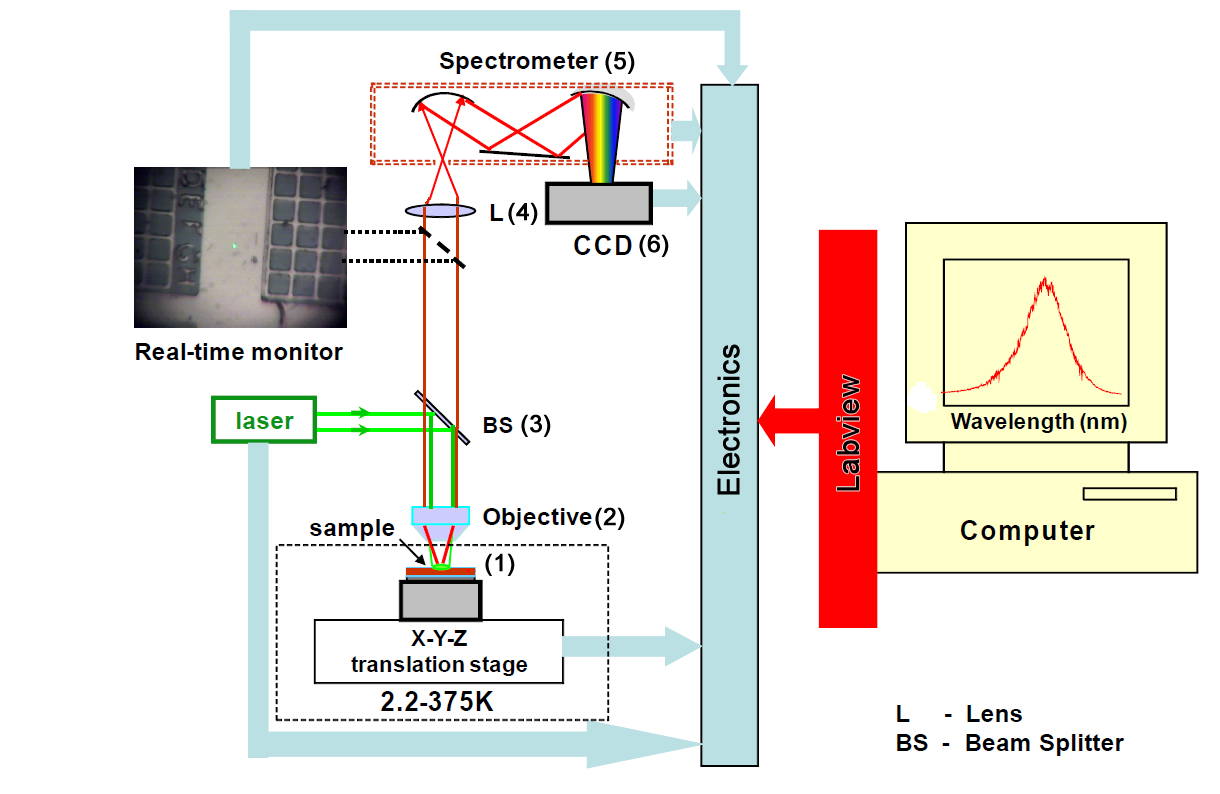
\includegraphics[width=\columnwidth]{lab_setup}%
\caption{Lab setup}%
\label{fig:lab_setup}%
\end{figure}



\begin{table}[H]
\centering
\begin{tabular}{|c|c|c|c|}
\hline
\textbf{\#} & \textbf{Part} & \textbf{Product \#} & \textbf{Manufacturer} \\
\hline
1 & Cryostat & Janis ST-500 & Janis Research Company \\ \hline
2 & Objective & NT56-982 & Edmund Optics \\ \hline
3 & Beam splitter & BS017 & Thorlabs \\ \hline
4 & Lens & ACN127-020-B & Thorlabs \\ \hline
5 & Spectrometer & iHR550 Imaging Spectrometer & Horiba Scientific \\ \hline
9 & Camera & InGaAs Spectroscopy CCD & Andor Technology \\ \hline
\end{tabular}
\caption{Lab setup optical components}
\label{tab:lab_setup}
\end{table}

\subsection{Pumping wavelength}

Pumping light needs to have enough energy to fill all available states in the crystal lattice, in order to detect defects and impurities. For silicon, which has a bandgap of around 1.1eV, has most impurity/defect bands below the bandgap. In order to fill these states, the pumping wavelength should be below 1125nm, which corresponds to energies just over 1.1eV.

Silicon has different absorption lengths for different wavelengths. For 1125nm, the absorption depth is nearly 200~$�$m \cite{laserdybde}. Compared to absorption for 532nm, 1125nm reach 200 times deeper into the sample.

Absorption length of about 1~$�$m for 532 nm laser, means that iron precipitates deeper in the sample won't be detected \cite{gundel09}. This limitation might be overcome by an excitation laser with a longer wavelength and absorption length in silicon. \cite{lee09} report that small angle grain boundaries in multicrystalline silicon of 1$^\circ$-1.5$^\circ$ show D3 and D4 lines, while 2$^\circ$-2.5$^\circ$ show D1 and D2 lines. Comparing to data from electron beam induced current measurements show D1 and D2 lines to be correlated with shallow levels, while D3 and D4 appear in both shallow and deep levels \cite{lee09}.

A pumping wavelength of 800 nm is chosen for excitation. This corresponds to an absorption depth of 12~$�$m in silicon. With a larger wavelength, it would be invisible to the naked eye, and make it much more difficult to align the setup, and make sure nothing is blocking the pathway. In the case of an imperfect filter in front of the spectrometer, 800nm (1.55eV) and the second order diffraction maxima at 1600~nm (0.775~eV) would be outside the most interesting wavelengths from silicon luminescence (see table \ref{energy_bands}).

\subsection{Spot size}

Having a small diameter on the pumping laser allows for a high resolution of characteristics on the sample. In an iron contaminated sample, \cite{gundel09} show that at some distinct spots of a size between 1$�$m and 4$�$m, the band to band photoluminescence peak is particular low at spots with iron precipitates. 

A large electron hole droplet could overshadow characteristics from impurities in the sample. \cite{satoshi04} show that electron hole droplets become more intense for a smaller volume, with a silicon nanolayer smaller than the absorption depth of the laser. \cite{satoshi04} used a 488nm pumping laser with 1,5$�$m diameter, on silicon nanolayer thickness of 50nm and 340nm. For the 50nm layer, \cite{satoshi04} observed a large electron hole droplet, even for small pumping intensities, with the same amount of photo excited carriers per volume as for the 340nm layer. Assuming that a small volume give rise to a larger electron hole droplet, it would be a limiting factor for the spot size and pumping wavelength.

For the setup given here, the spot size is around 2~$�$m.

\subsection{Laser intensity}

With a large pumping intensity, an electron hole droplet become visible in the specter around 1.08eV in bulk silicon \cite{hammond75}. \cite{satoshi04} show that electron hole droplets occur at weak excitations (0.75mW) and even at high temperatures for a silicon nanolayer of 50nm. For thickness of 340nm, the electron hole droplet show up at pumping intensity of 3mW and above, and the intensity of the electron hole droplet grow larger than for the free exciton at 15mW. This electron hole droplet is not wanted, as it can mask characteristic photoluminescence from impurities.

With a larger pumping intensity, the impurity photoluminescence would in some cases also increase. Photoluminescence from chromium bound with a boron atom is known to increase linearly with laser power \cite{conzelmann82,conzelmann83}, and would be easier to detect at a higher pumping intensity.

%%%%%%%%%%\subsection{Temperature}

\subsection{Expected results}

\subsubsection{Phosphorus and boron doped samples}

With fairly high concentrations of doping atoms, it's expected that they show up as separate lines in the photoluminescence spectra. \cite{dean67} observe a line around 1.0924eV which is attributed to B$^{TO}$. Concentrations values for B in \cite{dean67} are $6*10^{16}$~cm$^{-3}$. Also observed is a phosphorus line at 1.0916eV, with 8*10$^{16}$cm$^-3$ phosphorus atoms. ES1 and MH2 have similar B and P values, and is expected to show the same behavior. (See figure \ref{fig:boronSiPL} and \ref{fig:PSiPL} in appendix \ref{appendix:tabeller})

There is a photoluminescence line involving carbon bound to oxygen in Czochralski silicon known as the C-O band \cite{davies88}. In \cite{hare72}, it was observed only in crucible grown silicon, but not in float zone. In the crucible grown silicon, the oxygen impurities where 2\cdot10$^{18}$~atoms/cm$^3$, which is over ten times more than in ES1 and MH2. This makes it unlikely that any C-O complex luminescence will be strong enough to be detectable in these samples.

Another line involving carbon, is the two-carbon atom band \cite{davies88}. This band has been detected in float-zone silicon with C = 9.7\cdot10$^{16}$~cm$^{-3}$ after irradiation, together with the C-O complex line. The relative intensity between the C-O band and the two-carbon atom band in \cite{davies88} show that the 969~meV band is close to 5 times larger than the 789~meV band. With both MH2 and ES1 having carbon impurities around 6\cdot10$^{17}$~cm$^{-3}$ it is possible that this line at 969~meV will be visible. 

As for aluminum, \cite{dean67} show a line at 1.09~eV called Al$^{TO}$ in a sample with 2\cdot10$^{16}$cm$^{-3}$ Al doping atoms. In ES1 and MH2, the Al impurities are 20 times less. In addtion to a fairly low value of Al impurities, the Al$^TO$ line is very close to the I$^{TO}$, which can make it difficult to detect, and not likely to show up in the results.

Fe bound with boron is also known to give rise to photoluminescence \cite{mohring83}. The sample used in the article had  10$^{13}$ to 10$^{16}$~cm$^{-3}$ boron doping concentration. The article doesn't mention how many Fe impurity atoms that's introduced into the sample, but it's done by high temperature diffusion, and assumed to be considerably larger than for all the samples in this study. 

Based on the low values of Fe impurities in these samples, it's assumed that interstitial Fe won't have any effect on the photoluminescence bands. The same goes for Ti, which also have a very low amount present.


\subsubsection{Sample with added Chromium}

This sample have the same impurity values as ES1, except for chromium. The closest comparison is samples used in \cite{conzelmann82}. Here, luminescence spectra was observed for chromium in an p-type sample. Interstitial chromium concentrations where between $10^14$ and $10^16 atoms/cm^-3$ in \cite{conzelmann82}.

Chromium in an n-type sample doped with phosphorus atoms does not result in any luminescence, but chromium bound with boron show a clear line at 0.8432eV (CrB$^0$). The reaction velocity for the formation of CrB pairs at room temperature depend on the boron concentration. For large (10$^15$cm$^-3$) boron content, the chromium-boron reaction reach saturation in less than a day after chromium diffusion \cite{conzelmann82}.

MH2 are neither n og p-type, however there is enough boron atoms to saturate chromium by forming CrB pairs. Chromium atoms are in the order of 10$^{14}$~atoms/cm$^3$ which is similar to that in \cite{conzelmann82}. Expected photoluminescence spectra is therefor expected to be similar. (See figure \ref{fig:CrBSiPL} in appendix). With most of the boron bound with chromium, it is likely that the boron lines will be severely reduced compared to ES1, and not detectable. There are also Fe impurities present in the sample, that can form bonds with boron. Based on the low amount of Fe in this sample, those bonds are not believed to have any impact on the photoluminescence.

\subsubsection{Sample from clean feedstock}

Having carbon values around 2.26\cdot10$^{17}$, it is possible that the two-carbon atom band is visible here also. Else this sample is expected to only show intrinsic values similar to \cite{dean67} in so called "`good"' areas due to low concentration of impurities. However, there might be precipitates and higher concentration of impurities at the grain boundaries and dislocations. Particularly heavy metals like Fe and Al can be detected here. It is expected that the band to band recombination from silicon show considerably lower intensity for these areas.

\subsection{Results plotting}
In order to plot the results from the spectrometer, there are a few manipulations that's needed.

\subsubsection{Disregarding defect pixels}

By taking a spectra with the shutter closed, it is possible to measure the dark current coming from the camera. The dark current should be equally distributed across the pixels, based on the assumption that all pixels behave the same. For long integration time, this is not the case:

\begin{figure}[H]
\centering
\includegraphics[width=\columnwidth]{Dark_current-40s}
\caption[Defective pixels]{Dark current signal from the camera with defective pixels with shutter closed, and CCD at -75$^\circ$C using a random center wavelength}%
\label{fig:dark_current_40s}%
\end{figure}

To solve this problem, the four pixels are disregarded, and the value of the neighbor pixel has been used instead. Matlab code for this is available in the appendix. Comparing the before and after clearly show how this is done:

\begin{figure}[H]
\centering
\includegraphics[width=\columnwidth]{Dark_current-40s_corrected}
\caption[Defective pixels corrected]{Dark current signal from the camera with defective pixel correction in red using a random center wavelength}%
\label{fig:dark_current_40s-corrected}%
\end{figure}

The defective pixels are less apparent for shorter integration time, but still a problem:

\begin{figure}[H]
\centering
\subfigure[Dark current without correction]{
\includegraphics[width=.45\columnwidth]{Dark_current-10s}
\label{fig:dark_current_10s}
}
\subfigure[Dark current with correction (red)]{
\includegraphics[width=.45\columnwidth]{Dark_current-10s_corrected}
\label{fig:dark_current_10s-corrected}
}
\label{fig:dark_current_correction_10s-parentfig}
\caption[Dark current with 10s integration time]{Dark current with 10s integration time using a random center wavelength}
\end{figure}

Dead pixel correction is performed in all results.

\subsubsection{Noise reduction}

As seen in the previous section, there is a dark current offset present. Ideally, all pixels should behave exactly the same, and give rise to the same dark current offset. If all pixels behaved the same, and with the same variance in between measurements, it could simply be subtracted. This is not the case. The dark current is unevenly distributed over the pixel array, and needs to be measured by itself in order to remove it. The mean dark current noise shape is pretty much the same from measurement to measurement using the same CCD temperature. In addition to the mean offset, there is white noise elements. 

\begin{figure}[H]
\centering
\includegraphics[width=\columnwidth]{Dark_current_and_background_noise-20s}
\caption[Dark current and noise]{Dark current (blue) and dark current + background noise (red) with Savitzky-Golay filtered noise floor estimation (cyan)}%
\label{fig:dark_current_and_background_noise}%
\end{figure}

By subtracting the mean offset found in the dark current noise measurement, only background noise and white noise would be left. The matlab code used to do this can be found in the appendix.

\begin{figure}[H]
\centering
\includegraphics[width=\columnwidth]{Dark_current_removed-20s}
\caption[Dark current removed]{Dark current removed from background noise (blue), and Savitzky-Golay filtered signal (cyan)}%
\label{fig:dark_current_removed-20s}%
\end{figure}

It appears that the dark current noise is larger with the shutter open, compared to closed. But a more critical noise in the spectrum is a background signal around 1064nm. The spectrometer has a range of 140nm when using 300 as grating. It has proven difficult to align the system so that the entire array of pixels in the camera get an equally distributed light beam. And based on the noise level, the nm interval is chosen as 100nm, in order to remove the left hand side of the spectra when gluing different intervals together. This also avoid the problem of not hitting the entire array evenly. To get a full overview over the background noise, a full spectra was done, and glued together. This full spectra show that the artifact visible in \ref{fig:dark_current_removed-20s} is the only background noise line visible in the wavelength area 800-1650nm.

\subsubsection{Savitzky-Golay filtering}

Savitzky-Golay filter (also called digital smoothing polynomial filter or least-squares smoothing filter), is a smoothing filter which essentially performs a local polynomial regression on a series of values equally spaced. This filter is chosen because of the large frequency span of the signal. Although Savitzky-Golay filters are more effective at preserving the pertinent high frequency components of the signal, they are less successful than standard averaging FIR filters at rejecting noise \cite{signal_processing}.
